
\subsubsection{DCT Transform}
DCT transformation like fourier transform, intends to reduce existed redundancy in the frequency domain. The equations of two dimensional discrete cosines transform (DCT), And inverse discrete cosine transform (IDCT), are given below in order.
\begin{align}
    F(u,v) &= \sqrt{\frac{2}{MN}}C(u)C(v)\sum_{x=0}^{M-1}\sum_{y=1}^{N-1}f(x,y)cos[\frac{\pi}{2N}(2x+1)u]cos[\frac{\pi}{2M}(2(y+1)v)] \\
    f(u,v) &= \sqrt{\frac{2}{MN}}\sum_{x=0}^{M-1}\sum_{y=1}^{N-1}C(u)C(v) F(x,y)cos[\frac{\pi}{2N}(2x+1)u]cos[\frac{\pi}{2M}(2(y+1)v)]
\end{align}
where $M$ and $N$ are sizes of the image. And 
\begin{align}
    C(u) = \begin{cases}
    \frac{1}{\sqrt{2}}, \quad u=0;\\
    1, u=1,2,...N-1;
    \end{cases}
\end{align}

\begin{figure}[!htbp]
\centering
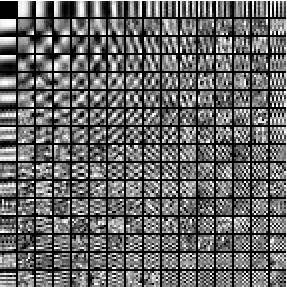
\includegraphics[width=0.2\linewidth]{images/DCT_dict.png}
\caption{A standard discrete cosine (DCT) dictionary;}
\label{dic1}
\end{figure}

\begin{algorithm}[!htbp] 
\caption{Block-sparse Dictionary Update}
\label{alg:Framwork} 
\begin{algorithmic}
\REQUIRE ~~\\%Input
The input signal $\mathbf{Y}$, block sparsity level $k$, and maximal block size $s$.\\
\ENSURE ~~\\ %Output
Learned Dictionary $\mathbf{\Phi}$ with optimal block struture $d$.\\
% --------------------------------------------------------\\
\STATE 1. Initialise the dictionary $D(0)$ as the outcome of K-SVD.\\
\STATE 2. For $N$ number of iterations.\\
\STATE \quad - Fix dictionary $\mathbf{\Phi}^{(m-1)}$ and update coefficients $x^{m}$ and block structure $d^{(m)}$ by applying sparse agglomerative clustering.\\
\STATE \quad - Fix the block structure $d^(m)$ and update the dictionary atoms $\mathbf{\Phi}^{(m)}$ by applying BS-SVD.\\
\end{algorithmic}
\end{algorithm}
